\section{Generación de Lenguaje Natural}\label{s:nlg}
Como se ha descrito y observado gracias a la tabla \ref{tab:dailymail}, el tráfico de correos electrónicos diarios continúa en constante crecimiento hasta llegar, al menos, a la gigantesca cifra de 376 mil millones enviados al día en todo el mundo. Esto se revierte en una gran cantidad de tiempo invertido para la redacción de todos estos mensajes que no se mandan de manera automática. Sin embargo, esta gran dedicación al e-mail lleva produciéndose desde hace más de una década, cuando no nos encontrábamos con cifras de tráfico tan elevadas. Según \cite{mckinsey}, de media los empleados invertían el 28\% de su tiempo semanal en la gestión del correo electrónico (como viene reflejado en la figura \ref{fig:e-mailwork}). Esto se traduce en más de once horas dedicadas única y exclusivamente a leer y contestar mensajes, enviando y recibiendo una media de 124 e-mails por día \citep{radicati2015email}. Por si estos datos no fueran suficientemente preocupantes, de cara a la productividad laboral y resolución eficiente de las tareas, según \cite{forbes} este problema se ha agravado en los últimos años por diversas causas (entre las que se encuentra la pandemia de la Covid-19). En definitiva, hoy en día podemos afirmar que tanto en el ámbito profesional como personal se invierte una gran cantidad de esfuerzo y tiempo para gestionar nuestra cuenta de e-mail, lo cual plantea un problema en el que vemos que, en lugar de ser una herramienta útil, se convierte en una responsabilidad más que debe llevarse al día y de la que no es posible desprenderse ya que la capacidad de mandar estos mensajes es imprescindible para llevar a cabo tareas del día a día. Pero, ¿y si fuera posible ahorrar todo este tiempo de escritura de correos electrónicos?

\begin{figure}[h]
	\centering%
	\centerline{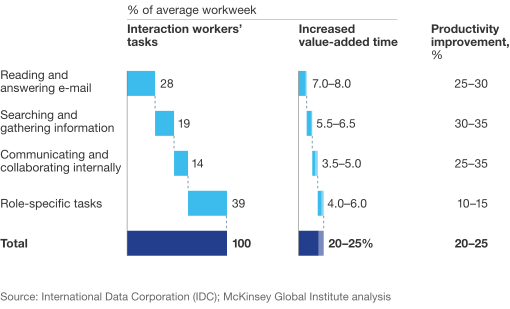
\includegraphics[width = 0.9\textwidth]{Imagenes/Bitmap/mckinsey.png}}%
	\caption{Porcentaje de tiempo de un trabajador dedicado a cada tarea}%
	\label{fig:e-mailwork}
\end{figure}

Para lograr este propósito es imprescindible profundizar en la rama de la Inteligencia Artificial conocida como \textit{Generación de Lenguaje Natural} (cuyas siglas son \textit{NLG} por su nombre en inglés \textit{Natural Language Generation}). Un buen ejemplo de aplicación de las técnicas de generación automática de textos son los 100.000 libros que Philip M. Parker puso a la venta en la plataforma \textit{Amazon.com} incluyendo títulos de temáticas tan variadas como \textit{El libro oficial del paciente sobre la estenosis espinal} \citep{parker2002official}, \textit{Perspectivas mundiales de 2009 a 2014 de los envases de 60 miligramos de Fromage Frais} \citep{parkerfromage},  \textit{Perspectivas de 2007 a 2012 de las tapetes de nudo, alfombras de baño y conjuntos que miden 6 pies por 9 pies o menos en la India} \citep{parkerrugs} y \textit{Tesauro Quechua - Inglés} \citep{parkerquechua}.

Resulta evidente que dicha cantidad de libros no pudieron ser escritos por Parker, sino que debió hacerse uso de técnicas de generación automática de textos. El algoritmo utilizado para dicho propósito, se engloba dentro de los métodos de generación conocidos como \textit{text-to-text} (texto a texto en castellano), dado que este tipo de técnicas toman como entrada textos ya existentes (normalmente escritos a mano y no generados automáticamente) y producen un nuevo texto coherente como salida. Otras aplicaciones de este tipo de métodos son la traducción automática de un idioma a otro \citep{hutchins2009introduction, oettinger2013automatic}, el resumen automático de textos \citep{mani2001automatic, nenkova2011automatic}, la simplificación de textos complejos, ya sea para hacerlos más accesibles para un público de lectores de bajo nivel de alfabetización \citep{siddharthan2014survey, bautista2011empirical} o niños \citep{macdonald2016summarising}, corrección automática de ortografía, gramática y texto \citep{kukich1992techniques, ng2014conll}, generación automática de revisiones de artículos científicos \citep{bartoli2016your}, generación de paráfrasis dada una frase de entrada \citep{bannard2005paraphrasing}, generación automática de preguntas con fines didácticos y educativos \citep{brown2005automatic}, generación automática de relatos dada una descripción conceptual de la historia deseada \citep{gervas2004story} o reescritura de textos (en concreto correos electrónicos) con estilo en función del destinatario \citep{mitfg}.

Además de estos métodos text-to-text, existen los llamados \textit{data-to-text} (datos a texto), en los cuales en lugar de recibir un texto como entrada, se genera el lenguaje a partir de datos. Estos pueden ser de todo tipo para dar lugar a informes o resúmenes como pueden ser de índole climatológica \citep{goldberg1994using, ramos2014linguistic}, financiera \citep{plachouras2016interacting}, ingenieril, como por ejemplo el trabajo desarrollado por \cite{yu2007choosing} para generar resúmenes de datos recopilados por sensores en turbinas de gas, sanitaria \citep{huske2003text, banaee2013towards}, como la investigación llevada a cabo por \cite{portet2009automatic} para obtener informes textuales a partir de datos de cuidados intensivos neonatales, o, incluso, deportivos \citep{theune2001data, chen2008learning}. Además de informes o resúmenes, también se utilizan los métodos \textit{data-to-text} para otros propósitos como la composición de discursos narrativos para relatos de varios personajes a partir de partidas de ajedrez \citep{gervas2014composing}, redacción de periódicos electrónicos a partir de datos de sensores \citep{molina2011generating}, generación de texto que aborda problemas medioambientales como el seguimiento de la fauna \citep{siddharthan2012blogging, ponnamperuma2013tag2blog}, la información medioambiental personalizada \citep{wanner2015getting} y la mejora del compromiso de los ciudadanos científicos a través de los comentarios generados \citep{van2016role} o producción de información interactiva sobre artefactos culturales \citep{stock2007adaptive}, entre otros.

Debido a que el objetivo de este trabajo se centra en la generación de correos electrónicos a partir del asunto, exploraremos en detalle las técnicas de Generación de Lenguaje Natural y, en especial, los métodos text-to-text. Para profundizar en los algoritmos y arquitecturas empleados ante los problemas de tipo data-to-text, conviene consultar la investigación llevada a cabo por \cite{gatt2018survey}, en la cual muestran el estado del arte de los trabajos realizados en este ámbito.

\subsection{¿Qué es la Generación de Lenguaje Natural?}
Dado que tanto los sistemas text-to-text como data-to-text y todas sus aplicaciones mencionadas anteriormente pertenecen a la rama de Generación de Lenguaje Natural, esta no debe definirse en función de la entrada del sistema, sino en la salida. Según \cite{biblia} la NLG es la conceptualización del ``campo de la inteligencia artificial y la lingüística computacional que se centra en los sistemas informáticos que son capaces de producir textos comprensibles en inglés u otra lengua humana. [...] Como área de investigación, la NLG presenta una perspectiva única ante problemas fundamentales de la inteligencia artificial, la ciencia cognitiva y la interacción. Estos incluyen cuestiones como por ejemplo cómo deben ser representados y cómo debe razonarse con la lingüística y el dominio del conocimiento, qué significa que un texto esté correctamente redactado y cómo es la mejor forma de comunicar información entre las computadoras y los usuarios.'' Por lo tanto, la Generación de Lenguaje Natural se puede definir como el ámbito que engloba el estudio de la producción de lenguaje no artificial, así como el diseño e implementación de algoritmos y sistemas computacionales cuyo resultado debe ser un texto que imite la forma en que los humanos se comunican verbalmente \citep{vicente2015generacion}, ya sea oralmente o por escrito \citep{del2007que}. Es decir, independientemente de la entrada recibida, se precisa el significado de NLG a partir de la salida esperada por el problema planteado. Tanto es así, que, como hemos visto, la entrada del sistema puede variar excesivamente \citep{mcdonald1993issues}: desde textos (que son precisamente los sistemas text-to-text) hasta datos de todo tipo como partidas de ajedrez \citep{gervas2014composing}, pictogramas \citep{gonzalez2019traductor} e, incluso, vídeos \citep{thomason2014integrating}. Sin embargo, autores como \cite{duvsek2020evaluating} acotan la definición de los sistemas de NLG estableciendo que la entrada deben ser representaciones semánticas, obviando así la primera tarea de la arquitectura propuesta por \cite{biblia} conocida como macro planificación o determinación del contenido (se explicará en la sección \ref{sss:realizer}), que es precisamente el punto en el que se generan dichas representaciones semánticas.

Cabe destacar que, aunque desde un principio hayamos diferenciado entre métodos text-to-text y data-to-text, ni los límites entre las dos aproximaciones ni la pertenencia de algunas técnicas a ellas se encuentran claramente definidos. Un ejemplo de ello podemos encontrarlo en la generación automática de resúmenes de textos. En principio se caracterizaría claramente como un sistema text-to-text. No obstante, al hacer frente a este problema se han desarrollado soluciones con las conocidas técnicas abstractivas \citep{genest2011framework}, que, como explican \cite{hahn2000challenges}, a diferencia de los métodos de extracción evitan recoger las frases completas y se limitan a tomar unidades semánticas. Este tipo de técnicas usadas, por ejemplo, en la obtención de opiniones de reseñas para la posterior generación de frases nuevas \citep{labbe2012towards}, también provienen de problemas data-to-text. A la inversa, un sistema data-to-text puede hacer uso de técnicas que principalmente son utilizadas en los casos de uso text-to-text \citep{mcintyre2009learning, kondadadi2013statistical}. Por otro lado, podría parecer que los métodos de \textit{deep learning} \citep{goodfellow2016deep} deben ser mayoritariamente utilizados en los problemas data-to-text utilizando el trabajo llevado a cabo por \cite{mikolov2013efficient}. Sin embargo, se han desarrollado extensamente esta clase de soluciones para la NLG con gran variedad de arquitecturas como las redes neuronales recurrentes \citep{cho2014learning, tang2016context}, muy a menudo combinadas con la memoria a corto plazo o LSTM \citep{chen2016enhanced}, o las arquitecturas conocidas como \textit{transformers} \citep{transformers}.

\subsection{Arquitecturas para la Generación de Lenguaje Natural}
Ante el problema de generación de lenguaje natural, se han propuesta diversas soluciones para abordarlo. Sin embargo, actualmente preponderan dos tipos de arquitecturas: la propuesta por \cite{biblia}, también conocida como arquitectura \textit{realizer} (toma el nombre de una de sus fases), que divide la generación en distintas subtareas y las aborda por separado, y la presentada por \cite{transformers}, también conocida como arquitectura \textit{transformer}, que expone una arquitectura constituida mayoritariamente por redes neuronales. Aunque en este trabajo hayamos hecho uso de esta última debido a la dificultad de establecer un dominio de lenguaje en los correos electrónicos, a continuación se hará una breve introducción a ambas.

\subsubsection{Arquitectura realizer}\label{sss:realizer}
A pesar de que en el trabajo de \cite{biblia} se centren principalmente en los sistemas de generación de lenguaje natural de tipo \textit{data-to-text}, esta arquitectura también ha sido utilizada por sistemas \textit{text-to-text} como para la generación automática de resúmenes a través de métodos abstractivos \citep{genest2011framework}. De hecho, incluso es posible hacer uso de la conceptualización de la entrada del sistema planteada por \cite{biblia} para este tipo de problemas.

La filosofía de esta arquitectura se centra en la modularización de las diferentes tareas a abordar durante la generación de lenguaje natural. De esta manera, cada módulo se enfrenta a un reto específico con el que debe lidiar y se conecta con el módulo anterior haciendo coincidir la salida del previo con la entrada del actual y, lo mismo, con el módulo posterior. Asimismo, se construye un \textit{pipeline} o arquitectura en secuencia de tareas con cada uno de los módulos.

La entrada de esta arquitectura viene determinada por una tupla de cuatro elementos $(k, c, u, d)$ donde cada uno de ellos puede representarse de distintas maneras. El primer elemento de la tupla es la \textit{base de conocimiento} (la letra viene dada por su denominación ingles \textit{knowledge source}). Se trata de la información acerca del dominio de nuestro sistema de generación de lenguaje natural, la cual suele consistir en un conjunto de bases de datos y bases de conocimiento, como las ontologías \citep{fensel2001ontologies}, que nuestra aplicación puede consultar durante su ejecución. Tanto la representación como el contenido de la base de conocimiento son altamente dependientes del tipo de aplicación que queramos construir, por ejemplo, en el trabajo de \cite{reiter2005choosing} la base de conocimiento consiste en parámetros meteorológicos numéricos de un modelo de predicción NWP, mientras que en el desarrollo presentado por \cite{reiter1995automatic} se utiliza como base de conocimiento un sistema de representación de conocimiento del mismo tipo que KL-ONE \citep{brachman1989overview} estructurado de manera jerárquica mediante relaciones \textit{is-a} y \textit{part-of}, del cual se pueden extraer diversas propiedades de las entidades que lo componen. Precisamente esta gran variabilidad en tan solo la primera componente de la entrada de la arquitectura realizer, es lo que sustenta la afirmación de \cite{biblia} de que no es posible proporcionar una caracterización formal genérica de lo que es una base de conocimiento y dificulta el establecimiento de esta componente en el sistema desarrollado si se hubiera elegido esta opción de arquitectura, ya que los correos electrónicos versan de una amplia variedad de temáticas muy distintas.

La segunda componente de la tupla de entrada es el objetivo de la comunicación (en inglés \textit{communicative goal}). Este describe el propósito del texto para el que se quiere generarlo. Es importante no confundirlo con el propósito general del sistema de generación de lenguaje natural. Por ejemplo, el objetivo final de sistema implementado por \cite{turner2007selecting} es generar resúmenes textuales de datos de predicción meteorológica numérica espacio-temporal. Sin embargo, su propósito comunicativo de una ejecución determinada es el de presentar predicciones meteorológicas de una localización geográfica y un momento temporal dados.

La letra u de la tupla se corresponde con el modelo de usuario (en inglés \textit{user model}), el cual consiste en una caracterización del receptor o público objetivo al que va dirigido el texto generado. Al igual que con el propósito comunicativo, no debe confundirse con los espectadores del sistema. Por ejemplo, el sistema implementado por \cite{reiter1999types} tiene como objetivo dirigirse a personas que consumen tabaco, ya que trata de generar cartas que convenzan a los pacientes con este hábito para que intenten superar su adicción. No obstante, no resulta adecuado utilizar el mismo tipo de técnicas de convicción y el mismo lenguaje para una persona que ha comenzado a fumar desde hace poco que a otra que lleva muchos años consumiendo tabaco. También, podría resultar interesante definir perfiles en función de la edad y otras características del paciente que permitirían personalizar aún más estas cartas. Son precisamente este tipo de propiedades las que englobaría el modelo de usuario que el sistema toma como entrada. No obstante, a pesar de que no existen demasiados ejemplos de trabajos que incluyan esta variable de entrada como lo desarrollan en su estudio \cite{goldberg1994fog}, por la dificultad de variación de los textos en función de dichos perfiles, este problema se suele tratar de abordar a través del estudio de la estilometría \citep{mitfg}.

El último componente de la entrada es la historia del discurso (en inglés \textit{discourse history}), la cual consiste en un modelo de la información transmitida y los temas tratados en el texto producido hasta el momento de la ejecución del sistema. Esto permite a la aplicación conocer las entidades y propiedades ya mencionadas gracias a las cuales es posible hacer un uso adecuado de los recursos anafóricos como los pronombres. En los sistemas de generación de lenguaje natural de interacción única, es decir, aquellos cuya ejecución produce un único texto con independencia de los generados en ejecuciones previas, la historia discursiva comienza como una estructura de datos vacía y se construye y utiliza durante la redacción del texto a generar. Todo lo contrario son los sistemas de diálogo, como los \textit{chatbots}, en los cuales la historia del discurso suele hacer referencia al registro de diálogo, utilizado como repositorio de información sobre las interacciones previas entre el usuario y la aplicación de NLG. En trabajos como el desarrollado por \cite{milosavljevic1996text}, en el cual se espera que los usuarios interactúen con una serie de textos relacionados, la historia discursiva resulta ser una mezcla de la utilizada en los sistemas de interacción única con la preponderante en los sistemas de diálogo. De esta manera, esta última componente de la tupla de entrada facilita el hacer referencias en el nuevo texto a entidades o conceptos mencionados en el texto actual o previos, o utilizar marcadores discursivos como ``como se ha mencionado anteriormente'' en momentos en que el texto generado repite información ya presentada en los anteriores.

Aunque puede resultar obvio, es importante tener en cuenta que, en la mayoría de los casos, será necesario un preprocesado del texto o los datos de entrada (sobre todo si han de ser analizados e interpretados) para facilitar el trabajo a la arquitectura presentada por \cite{biblia}, de manera que sea más sencillo utilizar la entrada en cada una de las fases \citep{han2011data}. Este primer preprocesado es plenamente opcional y depende del origen de la entrada que se vaya a utilizar.

Una vez se conoce la entrada y salida establecida para un sistema de generación de lenguaje natural, se puede comenzar la presentación de la arquitectura modular secuencial. Según \cite{biblia}, el proceso de generación puede descomponerse en tres fases: la macro planificación, la micro planificación y la realización (que da nombre a la arquitectura por ser la última fase). Los módulos que implementan cada una de ellas se conectan entre sí como muestra la figura \ref{fig:pipelinenlg}.

\begin{figure}[h]
	\centering%
	\centerline{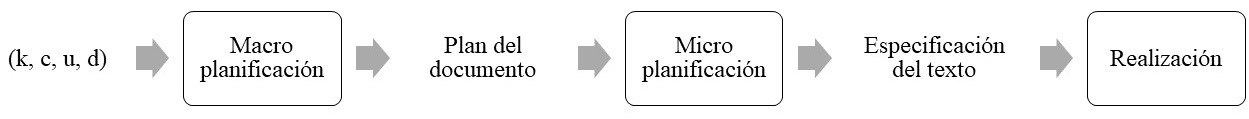
\includegraphics[width = \textwidth]{Imagenes/Bitmap/pipeline-nlg.jpg}}%
	\caption{Arquitectura modular secuencial propuesta por \cite{biblia} para la NLG}%
	\label{fig:pipelinenlg}
\end{figure}

En términos generales, el trabajo del módulo de macro planificación es producir una especificación del contenido del texto y su estructura, mediante el uso del dominio y el conocimiento de la aplicación sobre qué información es la más adecuada teniendo en cuenta la tupla de entrada. Esta fase normalmente también requiere conocer cómo suelen estructurarse los documentos del dominio de nuestro sistema. Muchas de las técnicas empleadas para la implementación de la macro planificación suelen asemejarse a las utilizadas en el ámbito de los sistemas expertos.

Para que el texto sea coherente, es preciso estructurar el contenido del mismo en el orden correcto. Por este motivo, la salida del módulo de macro planificación, el plan del documento, suele implementarse como una estructura de datos, generalmente arbórea, donde en cada nodo se encapsula la información más importante que debe formar parte de un párrafo o frase, además de información de cómo se relaciona con el resto de nodos. Con el objetivo de generar esta salida, se dividen las tareas de este nodo en determinación del contenido y estructuración del documento.

La determinación del contenido es la primera tarea de la macro planificación y, por tanto, del proceso de generación. En ella el sistema decide qué información es relevante para ser incluida en el texto y cuál no. Por lo general, en los sistemas data-to-text, se puede extraer más información en los datos de la que se quiere transmitir y, por ese motivo, cobra importancia la capacidad de selección y existen numerosas investigaciones al respecto, como la de \cite{yu2007choosing}. Aunque la determinación del contenido está presente en la mayoría de los sistemas de generación de lenguaje natural \citep{mellish2006reference}, los enfoques suelen estar estrechamente relacionados con el dominio, de forma que se construye una estructura de datos ad hoc, cuyos elementos se denominan ``mensajes'' o también son llamadas ``representaciones semánticas'' por autores como \cite{duvsek2020evaluating}. Dicha estructura de datos se crea con el fin de especificar la salida de esta tarea (un ejemplo conceptual de un mensaje para un sistema que genera textos sobre la situación meteorológica puede observarse en la figura \ref{fig:messagenlg}). Este planteamiento de la determinación del contenido, dificulta el desarrollo de sistemas en los que el dominio es extenso, como es el caso de los correos electrónicos, ya que no es posible implementar una clase que englobe todas las casuísticas (como se verá en la sección \textcolor{red}{poner nº}, para resolver este problema se utilizará el concepto de \textit{Information Items} el cual pertenece al ámbito del resumen automático de textos). Sin embargo, sí se ha tratado de encontrar otro tipo de definición a la salida de esta tarea, como ocurre en el trabajo de \cite{guhe2007incremental}, el cual presenta una explicación cognitivamente plausible e incremental de la determinación del contenido, basada en estudios sobre las descripciones de observadores de eventos dinámicos a medida que se desarrollan.

\begin{figure}[h]
	\centering%
	\centerline{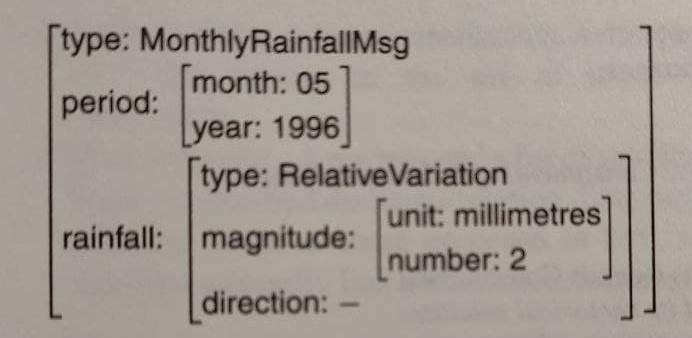
\includegraphics[width = 0.7\textwidth]{Imagenes/Bitmap/message-nlg.jpg}}%
	\caption{Ejemplo de mensaje}%
	Imagen extraída de \cite{biblia}
	\label{fig:messagenlg}
\end{figure}

La elección del contenido que debe ser expresado en el texto depende de varios factores, entre los que se encuentran: el propósito comunicativo, el modelo de usuario, las restricciones de la salida por limitaciones del dominio (como la longitud máxima que debe tener un texto) y la fuente de información (o base de conocimiento) subyacente disponible (es importante, aunque parezca evidente, no pretender generar información sobre la que el sistema no posee conocimiento o no es capaz de deducirlo con sus módulos de razonamiento correspondientes).

Como se ha mencionado anteriormente, además de la determinación del contenido, el módulo de macro planificación se encarga de abordar la tarea de estructuración del documento. Esta engloba todas las decisiones relativas a cómo cada parte del contenido debe ser agrupada en el texto y cómo debe ser relatada en términos retóricos. La estructura subyacente de un texto puede ser vista de manera jerárquica con los elementos textuales como cláusulas y las frases como constituyentes de largos fragmentos de texto, que son a su vez elementos de otros fragmentos más largos. Un texto puede ser analizado como una estructura arbórea cuyos elementos vienen relacionados por el tema que tratan (todas las frases sobre una misma temática podrían situarse en el mismo párrafo) y las relaciones discursivas (por ejemplo, es posible pasar de hablar en términos generales a entrar en detalles). Para abordar esta tarea la mayoría de trabajos, como el de \cite{williams2008generating}, suelen hacer uso de la llamada teoría de la estructura retórica \citep{mann1987rhetorical}, cuyas siglas son RST por su nombre en inglés \textit{Rhetorical Structure Theory}. La idea básica subyacente de la RST es que la coherencia y cohesión vienen dadas en virtud de las relaciones que mantienen los elementos del texto. También se pueden encontrar investigaciones, como es el caso de la realizada por \cite{mckeown1992text}, que lo resuelven mediante esquemas, es decir, patrones que determinan cómo se debe construir un documento a partir de elementos constituyentes que pueden ser mensajes o instancias de otros esquemas. Además, permiten incluir elementos opcionales que solo se incluirían cuando se cumplen ciertas condiciones de activación. Un ejemplo de implementación de los esquemas son las gramáticas independientes del contexto \citep{cremers1975context}.

En definitiva, el primer módulo de la arquitectura realizer es el de macro planificación, el cual construye primero los mensajes (seleccionando los datos, resumiéndolos si fuera necesario, razonando sobre ellos y adaptándolos en función de la tupla de entrada) y, a continuación, define una relación entre todos ellos (normalmente jerárquica), generando así lo que se conoce como plan del documento.

El plan del documento es la entrada del módulo de micro planificación, que es el encargado de las tareas de agregación (decidir cómo el plan del documento se convertirá en estructuras lingüísticas como frases y párrafos, y el orden de las mismas si esto no se ha resuelto en la tarea de estructuración del documento), lexicalización (decidir qué recursos lingüísticos, como palabras o construcciones sintácticas, serán utilizados) y generación de expresiones referenciales (decidir qué expresiones serán utilizadas para las distintas entidades). Por ejemplo, para un sistema de generación de reportes meteorológicos, el plan de documento podría especificar que en el texto debería incluirse el hecho de que en febrero de 2020 se observaron temperaturas por debajo de la media. No obstante, la decisión de como referirse a febrero de 2020 (existen numerosas opciones como ``el mes'', ``febrero'', ``febrero de 2020'', ``el segundo mes del año'', etcétera) es tarea del módulo de micro planificación. O también la salida de  la macro planificación puede añadir, además de la bajada media de temperaturas, un descenso en el mismo mes en la media de precipitaciones. Será entonces el módulo de micro planificación el encargado de determinar si estos dos hechos deben expresarse en frases separadas o combinados en una misma utilizando, quizás, la estructura de una oración coordinada copulativa.

Resulta razonable pensar que no cada mensaje generado en el plan del documento necesita ser expresado en una frase separado del resto. El hecho de combinar varios mensajes en una misma oración probablemente produzca un texto más fluido y legible \citep{dalianis1999aggregation, cheng2000capturing}. Precisamente esta decisión es la que se debe tomar en la fase de agregación, junto con la transformación de los mensajes en estructuras lingüísticas y elementos textuales más amplios como pueden ser los párrafos. Como explican \cite{biblia}, esta tarea no necesariamente precede a la de lexicalización, sino que suelen implementarse de manera que se ejecuten ambas en paralelo interactuando una con la otra, ya que suelen estar fuertemente relacionadas la elección de los términos a utilizar (lexicalización) y las estructuras lingüísticas empleadas.

En cuanto a la definición técnica de la agregación, esta tarea se ha interpretado de distintas maneras, desde la eliminación de redundancias hasta la combinación de las estructuras lingüísticas. Tanto es así, que \cite{reape1999just} hacen una distinción entre agregación a un nivel semántico y a nivel sintáctico. Esta fase se ha desarrollado ampliamente centrándose en las restricciones y reglas específicas del dominio de la aplicación, como es el caso de las investigaciones de \cite{hovy1987generating} y \cite{shaw1998clause}, aunque también se han implementado aplicaciones utilizando métodos dirigidos por corpus de ejemplos en los que las reglas se adquieren a partir de estos datos \citep{walker2001spot, stent2004trainable}.

La lexicalización, tarea del módulo de micro planificación, consiste en la elección de las distintas palabras (nombres, verbos, adjetivos y adverbios) que se requieren para expresar los distintos mensajes del plan del documento. La complejidad de este proceso radica en la cantidad de alternativas que el sistema de generación de lenguaje natural puede contemplar. A menudo, las restricciones contextuales (como intentar evitar la repetición de ideas o entidades) pueden ser de gran ayuda. Si el objetivo es generar textos con cierta variación \citep{theune2001data}, una solución puede ser elegir de manera aleatoria la opción de lexicalización. Sin embargo, puede ocurrir que aparezcan restricciones estilísticas o haya que tener en cuenta otras consideraciones como la actitud o postura afectiva acerca de lo que se está redactando \citep[Sección 5]{fleischman2002towards}. Este tipo de limitaciones dependerán del dominio de la aplicación.

Por otro lado, la lexicalización podría complicarse por dos razones \citep{bangalore2000corpus}: puede suponer la elección entre palabras de semántica similar, sinónimo o taxonómicamente relacionadas \citep{stede2000hyperonym, edmonds2002near}, y no siempre es sencillo modelar la lexicalización en términos de un mapeo nítido entre conceptos y palabras. Una fuente de dificultad es la imprecisión e inexactitud del lenguaje, que surge, por ejemplo, con términos que denotan propiedades que son graduables. Un buen ejemplo de ello es al seleccionar adjetivos como ancho o alto basado en las dimensiones de una entidad. Esto requiere que el sistema razone sobre la anchura o altura de objetos similares, pudiendo utilizar un estándar de comparación \citep{van2012not, kennedy2004scale}.

La otra tarea de la que se encarga el módulo de micro planificación es la generación de expresiones referenciales, la cual consiste en redactar expresiones que se refieran a las distintas entidades del texto que permitan al receptor identificar dicha entidad dado el contexto. Resulta un reto en la generación de lenguaje natural ya que hay distintas maneras de generar estas referencias, tanto la primera vez que se menciona la entidad (referencia inicial) como cuando esta es nombrada después de haber sido introducida en el discurso (referencia subsiguiente). Esta descripción de la generación de expresiones referenciales, puede parecer que guarda varias similitudes con la lexicalización, pero \cite{biblia} indican que la diferencia esencial entre ambas tareas es que, la que ahora atañe al texto, es ``una tarea de discriminación en la cual el sistema necesita comunicar suficiente información de cara a distinguir una entidad del dominio frente al resto de entidades'' evitando la ambigüedad. Esta fase de la micro planificación ha sido muy llamativa para varios investigadores como \cite{siddharthan2011information}, quienes han centrado sus esfuerzos en presentar diversas soluciones que permitan la implementación de esta tarea. La primera aproximación que se nos puede ocurrir es la llamada forma referencial, en la cual las entidades son descritas mediante pronombres, nombres propios o una descripción concreta. Esta elección depende, en cierta forma, en la medida en que la entidad se encuentre en el foco de atención de la estructura lingüística o se quiera destacar \citep{poesio2004centering}. De hecho, tales nociones subyacen a muchas investigaciones acerca de la generación de pronombres \citep{mccoy1999generating, callaway2002narrative, kibble2004optimizing}.

Precisamente elegir la forma referencial ha sido objeto de diversos trabajos, como el de \cite{belz2009generating}, sobre la generación de expresiones referenciales aprovechando el contexto que engloba lo que se quiere redactar, y la investigación de \cite{ferreira2017linguistic} que pone de manifiesto la problemática en la generación de nombres propios para las entidades.

Como puede observarse en la figura \ref{fig:pipelinenlg}, la salida del módulo de micro planificación es la especificación del texto. Se trata de un objeto que proporciona una definición completa y precisa del documento a generar. Análogo al plan de documento, la especificación del texto suele implementarse con una estructura arbórea en la cual las hojas son los objetos que \cite{biblia} llama especificación de oración (las cuales pueden conceptualizarse de distintas formas: fragmento de texto enlatado, estructura sintáctica abstracta o un frame de casos lexicalizados), mientras que los nodos internos suelen contener la información acerca de la estructura del documento en términos de párrafos, secciones, etcétera. La estructura que describe la especificación del texto es la estructura lógica del documento, no la física (cómo el material es distribuido a lo largo de las páginas, columnas, líneas), la cual es tarea del último módulo de la arquitectura realizer. En esta salida del módulo de micro planificación, no se suelen encontrar relaciones discursivas, los nodos internos normalmente no las especifican. Si fuera necesario comunicarlas, el módulo de micro planificación llevaría a cabo los cambios convenientes a nivel de especificación de oración. Otro dato importante de esta estructura de datos es que el orden de los constituyentes (los nodos hijos) está determinado por cómo se recorrerá el árbol de la especificación del texto.

Por último, el módulo de realización (por el cual se le da nombre a la arquitectura y es el que producirá el texto final) llevará a cabo las tareas de realización lingüística y realización estructural. La primera consiste en recibir las representaciones abstractas de las frases (especificación de oración), producidas en la micro planificación, y convertirlas en texto. Al igual que los documentos no son secuencias de oraciones ordenadas de forma aleatoria, las frases no son secuencias de palabras ordenadas al azar. Cada idioma se define, al menos en parte, por una serie de reglas que determinan cuándo una sentencia está bien construida. Dichas reglas son dirigidas por el campo de la morfología y la sintaxis. La realización lingüística suele definirse como el problema de aplicar reglas gramaticales a representaciones abstractas con el fin de producir un texto correcto a nivel sintáctico y morfológico. La complejidad de esta tarea dependerá entonces de cuán distinta sea la representación abstracta de su redacción final.

Para resolver el problema de realización lingüística, en el cual se debe ordenar y especificar los distintos constituyentes de una frase así como generar su correcta forma morfológica (incluyendo conjugación de verbos y concordancia de persona, género y número de las distintas entidades lingüísticas); se han propuesto distintas aproximaciones: plantillas preconstruidas, sistemas basados en la gramática preconstruidos y métodos estadísticos. La primera aproximación suele resultar de utilidad cuando el dominio de la aplicación es pequeño y la variación esperada es ínfima \citep{mcroy2003augmented}. Consiste en oraciones construidas previamente en las cuales solo es necesario rellenar ciertas entidades y ajustar algunas características morfológicas. La ventaja de las plantillas es que se tiene un control absoluto sobre la calidad de la salida y evita la generación de estructuras gramaticalmente incorrectas. Además, pueden utilizarse complejos sistemas de reglas para rellenar estos ``huecos'' haciendo que las plantillas sean difíciles de distinguir de otros métodos más sofisticados \citep{deemter2005real}. Las desventajas de esta aproximación son que se caracterizan por resultar excesivamente laboriosas si se construyen a mano, aunque se han desarrollado investigaciones para su generación automática a partir de corpus como la de \cite{angeli2012parsing} y la de \cite{kondadadi2013statistical}; y que no son una solución escalable para aplicaciones que requieran variaciones lingüísticas considerables.

Una alternativa a las plantillas son los sistemas en la gramática. Dichas gramáticas pueden ser construidas manualmente \citep{elhadad1996overview} o mediante inferencia \citep{parekh2000grammar} a través de corpus. La mayor dificultad de los sistemas basados en gramática es cómo tomar decisiones entre varias opciones válidas y relacionadas entre sí. La otra alternativa son los métodos estadísticos, en los que se pueden encontrar el aprovechamiento de técnicas como la gramática categórica combinatoria \citep{steedman2000}, como en el trabajo de \cite{espinosa2008hypertagging}, el método de construcción de árbol adyacente a la gramática \citep{gardent2015multiple} y todo tipo de técnicas de aprendizaje automático como las máquinas de soporte de vectores \citep{bohnet2010broad}, entre otros.

La última tarea es la denominada realización estructural. En ella se espera convertir las estructuras abstractas, como párrafos y secciones, en símbolos de marcado entendidos por el componente de presentación del documento (como por ejemplo las directivas HTML si se va a presentar en formato web). Algunos autores como \cite{gatt2018survey}, no consideran esta fase como parte de la arquitectura realizer. En cualquier caso, la salida del módulo de realización será el texto final generado.

En resumen, la arquitectura realizer consta de tres módulos: macro planificación, micro planificación y realización. El primero de ellos recibe una entrada en forma de tupla que incluye la base de conocimiento, el propósito comunicativo, el modelo de usuario y la historia del discurso. Con estos cuatro elementos, lleva a cabo las tareas de determinación del contenido y estructuración del documento, generando el plan del documento, que será la entra del módulo de micro planificación. Este último será el encargado de la agregación, lexicalización y la generación de expresiones referenciales, produciendo lo que se conoce como especificación del texto. Dicha entidad será recibida por el módulo de realización y ejecutará la realización lingüística y la realización estructural (cuando sea necesario), generando así el texto de lenguaje natural que se espera del sistema.

\subsubsection{Arquitectura transformer}\label{sss:transformer}
Como se ha señalado anteriormente, una de las grandes desventajas que presenta la arquitectura realizer, es su gigantesca dependencia del dominio del discurso en muchas de sus componentes. De hecho, la solución propuesta para implementar la determinación del contenido es una estructura de datos construida ad hoc, y esta es solo la primera fase de todo el pipeline. Esto no supone un problema cuando se plantea el desarrollo de sistemas de generación de lenguaje natural que pueden enmarcarse dentro de un ámbito específico (como los informes meteorológicos, las locuciones deportivas, etcétera). Sin embargo, cuando se busca generar correos electrónicos, el usuario podría plantearse escribir un e-mail sobre diversas temáticas muy variadas que resulta complicado restringir dentro de un campo semántico. Este tipo de problemas, dada su complejidad, suelen abordarse utilizando arquitecturas compuestas por redes neuronales \citep{goldberg2016primer}, normalmente de gran cantidad de capas ocultas (\textit{deep learning} o aprendizaje profundo).

La aplicación de las arquitecturas de redes neuronales en la NLG se remontan, al menos, al trabajo desarrollado por \cite{kukich1987phrases}. Desde entonces el interés por este tipo de soluciones comienza a despertar en la comunidad de inteligencia artificial y, concretamente, en el ámbito del lenguaje natural \citep{elman1990finding, elman1993learning, chang2006becoming}. Las redes neuronales están diseñadas para aprender representaciones a niveles crecientes de abstracción explotando la propagación hacia atrás \citep{lecun2015deep}, también denotada por su terminología inglesa \textit{backpropagation}. Estas arquitecturas son densas, de baja dimensión y distorsionadas, lo que las hace ideales para captar generalizaciones gramaticales y semánticas \citep{mikolov2013distributed, luong2013better, pennington2014glove}. Además han cosechado notables éxitos en la modelización secuencial utilizando redes \textit{feedforward} \citep{bengio2003neural, schwenk2005training}, modelos logarítmicos bilineales \citep{mnih2007three} y redes neuronales recurrentes \citep{mikolov2010recurrent}, incluyendo las RNN (redes neuronales recurrentes) a las que se les dota de unidades de memoria a corto plazo o LSTM \citep{hochreiter1997long}. Antes de que aparecieran en el panorama científico las arquitecturas transformers, estas últimas dominaban las soluciones de generación de lenguaje natural con redes neuronales, ya que su principal ventaja frente a otros modelos de lenguaje estándar es que compaginan la capacidad de hacer frente a secuencias de distintas longitudes y la de evitar tanto la escasez de datos como la explosión del número de parámetros. Precisamente una demostración del potencial de las redes neuronales recurrentes dotadas de unidades de memoria a corto plazo fue desarrollada en el trabajo de \cite{sutskever2011generating}.

El tipo de arquitectura que dio paso a los transformers, fue la conocida como \textit{Encoder-Decoder} \citep{sutskever2014sequence}, codificador-decodificador en castellano, cuya filosofía se basa en utilizar una red neuronal recurrente para codificar la entrada en un vector suficientemente representativo que será la entrada del decodificador, también implementado con una RNN. Esta distinción entre codificador y decodificador posibilita compartir el mismo vector de codificación entre diversas tareas de procesamiento de lenguaje natural \citep{dong2015multi, luong2015multi}. Además, facilita la adaptación del codificador con el fin de generar texto a partir de representaciones semánticas abstractas, al igual que se ha hecho en este trabajo tomando como referencia la investigación realizada por \cite{ferreira2017linguistic}.

A la arquitectura Encoder-Decoder hay que añadirle mecanismos de atención antes de llegar a la arquitectura transformer. Estos fuerzan al codificador, durante el entrenamiento, a darle más importancia (atribuyendo valores mayores en los pesos) a ciertas partes de la entrada del mismo de cara a la generación de determinados fragmentos de la salida en la decodificación \citep{tang2016context, xu2015show}. Esta técnica evita la necesidad de conectar neuronas de capas ocultas con la entrada, ya que los modelos de atención son capaces de aprender la correspondencia entre entrada y salida basado en fragmentos sueltos que representen a la entrada y textos de salida \citep{duvsek2016sequence}.

Es precisamente en el paradigma Encoder-Decoder y los mecanismos de atención en lo que se basa la conocida arquitectura transformer propuesta por \cite{transformers}, como puede observarse en la figura \ref{fig:transformer}. El rectángulo gris izquierdo de la imagen se corresponde con el codificador y el derecho con el decodificador. Dentro de ambos se pueden identificar módulos de atención. Expliquemos en detalle en qué consiste este modelo.

\begin{figure}[h]
	\centering%
	\centerline{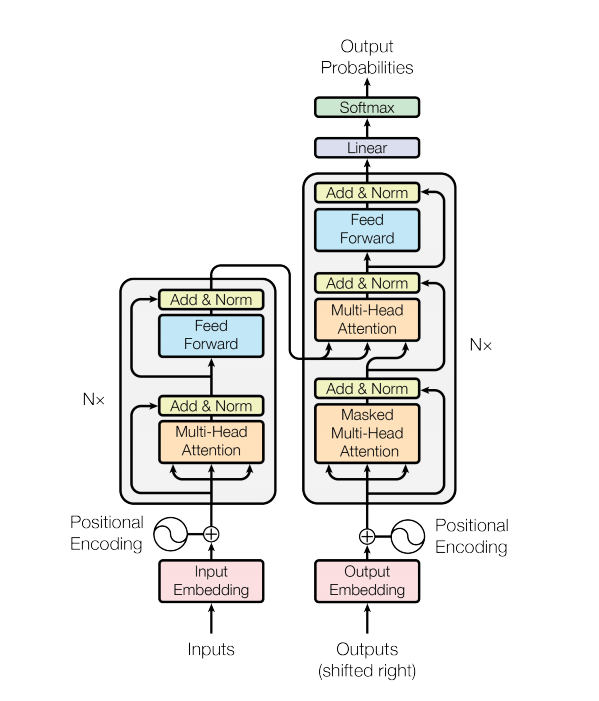
\includegraphics[width = 0.75\textwidth]{Imagenes/Bitmap/transformer.png}}%
	\caption{Modelo de arquitectura transformer}%
	Imagen extraída de \cite{transformers}
	\label{fig:transformer}
\end{figure}

Como se ha explicado anteriormente, la entrada de la arquitectura transformer (que puede ser un texto que debe completar añadiendo al final la composición lingüística correspondiente, un documento del que se espera obtener un resumen, un texto que quiere traducirse, ...) será responsabilidad del codificador (parte izquierda de la imagen). Tras haber pasado por este módulo, se enviará al decodificador, el cual, como puede observarse en la figura, también tiene otra entrada distinta. Además de recibir la salida del codificador, el decodificador será informado de toda la secuencia de texto generada anteriormente, de manera que durante el entrenamiento, se evaluará su rendimiento palabra a palabra de cada uno de los textos que se espera que produzca y se llevará a cabo el backpropagation en función del token que debe dar como resultado. En la primera iteración de un ejemplo de entrenamiento, momento en el que no se ha generado ninguna palabra, el decodificador recibirá como entrada un token especial que indicará el inicio de un texto (también existirá otro para determinar el final que deberá ser generado por la arquitectura). Por ejemplo, si se entrena el modelo con citas famosas de películas que estén incompletas, cuyo objetivo es acabarlas, y se quiere completar la famosa intervención del protagonista de la película \textit{Forrest Gump} ``Mamá siempre decía que la vida era como una caja de chocolates. Nunca sabes qué te va a tocar'' a partir de la primera parte ``Mamá siempre decía que la vida era como una caja de chocolates.'', la entrada de la arquitectura (que pasará al codificador) será siempre la tokenización (acción de transformar texto a vectores numéricos) de dicha primera parte. Por otro lado, en la primera iteración, la entrada adicional del decodificador será el token especial de inicio (en la literatura suele denotarse por \textit{<start>}). De esta manera, tras pasar por el decodificador, la salida que se obtendrá se corresponderá con un vector con tantas componentes como palabras compongan el vocabulario de salida (que no necesariamente es el mismo que el vocabulario de entrada, como en el caso de los traductores). Cada elemento de dicho vector indicará la probabilidad de que sea la palabra que le corresponde la siguiente en generar. Asimismo, se escoge el token con mayor probabilidad y ese es el que es incluye al texto. 

Supongamos que el transformer entrenado de ejemplo es suficientemente bueno y ha generado la palabra correcta: ``Nunca''. Entonces, con la misma entrada del codificador, se vuelve a llamar al modelo, pero esta vez, dándole como parámetros de entrada al decodificador la tokenización resultante al concatenar el token especial de inicio y la palabra ``Nunca''. Si el resultado es ``sabes'', se continuará manteniendo la entrada del codificador y facilitándole al decodificador la tokenización de ``<start>Nunca sabes''. Este proceso se repite hasta que el transformer generar el token especial de fin (normalmente denotado por \textit{<end>}). En resumen, si facilitándole a nuestro modelo la entrada ``Máma siempre decía que la vida era como una caja de chocolates.'' se desea obtener ``Nunca sabes qué te va a tocar'', la entrada de codificador será siempre la tokenización de ``Máma siempre decía que la vida era como una caja de chocolates.'', y la del decodificador será la tokenización de ``<start>'' la primera vez, luego ``<start>Nunca'' (si ha generado la palabra ``Nunca'') en la segunda iteración, después la entrada del decodificador será la tokenización de ``<start>Nunca sabes'' (si ha producido la palabra ``sabes'' en la iteración anterior) y, así sucesivamente, se le añadirán los tokens generados en la iteración anterior hasta que el modelo produzca el token ``<end>''.

Una vez se ha comprendido lo que la arquitectura espera como entrada de sus módulos, se procede a entrar en detalle de las distintas partes de la misma, comenzando por las capas de \textit{Embedding} \citep{mikolov2013efficient}. Como se ha dicho anteriormente, no es posible dar como entrada del modelo valores de tipo texto, por lo que es necesario transformarlo a formato numérico. Existen distintas opciones para llevar a cabo esta conversión: asignación de números arbitraria, codificación \textit{one-hot-encoding}, etcétera. Independientemente de la elegida, la representación de los tokens acarreará consigo problemas como la inconsistencia entre las relaciones numéricas como la distancia y las relaciones semánticas de las palabras a las que se corresponden (en el caso de la asignación arbitraria) o la equidistancia entre todas las codificaciones entre sí (en el caso del one-hot-encoding). Por este motivo, es necesario utilizar la capa de embeddings, la cual consiste en una red neuronal que, a partir de la tokenización elegida, produce vectores de cada uno de los tokens y ajusta sus pesos en función de la finalidad del sistema. De esta manera, no solo se contempla la semántica de las distintas palabras pudiendo calcular su similitud hallando la distancia entre los vectores que las representan o el ángulo entre ambos, sino que también se genera un espacio n-dimensional (donde n es el tamaño de los vectores de salida, por lo general en los transformers se elige 512) en función del propósito de la red neuronal en el que cada dimensión determina una característica diferente de las palabras.

Sin embargo, como la capa de embeddings transforma token a token independientemente de su posición en el texto de entrada, el vector de salida (llamado vector embedding) no contará con dicha información que es necesaria, ya que, a diferencia de las redes LSTM que computan los tokens secuencialmente, los transformers, para ser más eficientes, procesan todos los vectores embedding a la vez. La razón por la que es recomendable tener en cuenta la información de la posición de cada token, es que la semántica de un texto puede verse drásticamente modificada en función de dicho orden. Por ejemplo, las frases ``aunque no ganara el premio, estaba satisfecha'' y ``aunque ganar el premio, no estaba satisfecha'' comparten los mismos tokens, no obstante, el orden de estos, en concreto de la palabra ``no'', cambia completamente el significado y resulta una información crítica para entenderlas y diferenciarlas. Por esta razón, a los vectores embeddings, se le suman representaciones vectoriales (vectores de posición) de la posición del token con el que se corresponden, obteniendo así lo que se llama embeddings de posición. La pregunta es entonces, qué vectores se le deben sumar a los vectores embeddings y cómo deben construirse. Una primera idea podría ser que los vectores de posición constaran de todos los elementos iguales indicando el índice de la palabra en el texto (la primera palabra tendría un vector nulo, la segunda un vector con todos los elementos 1, la tercera sería un vector lleno con 2, y así consecutivamente). Desgraciadamente, esta solución no funciona correctamente, ya que la suma distorsionaría mucho los vectores embeddings producidos, especialmente aquellos que aparecen más tarde en el texto (por ejemplo, un texto de 100 palabras le sumaría a cada elemento del vector el gigantesco número 99, lo que introduciría mucho ruido).

Una solución que evita esta gran distorsión podría ser la de sumar vectores con todos los elementos iguales cuyos valores sean fracciones menores que 1. Una implementación de esta solución sería que el valor repetido que se le va a sumar a todas las posiciones de cada vector embedding sea $p/(N-1)$ donde $p$ es la posición del token en el texto (comenzando por 0) y $N$ el número de tokens del mismo. Sin embargo, este apaño produciría vectores de posición distintos para token en el mismo lugar, pero en textos con distinta longitud. Probablemente esto generaría confusión en el modelo, complicaría su entrenamiento y reduciría su precisión. Quizás se podría arreglar definiendo $N$ como una constante que sea la longitud máxima de un texto de entrada aunque el que se utilice sea más corto, pero este hecho evitaría que hubiera gran diferencia entre el comienzo y el final de un documento cuando su longitud es considerablemente más pequeña que la $N$ elegida. Como consecuencia de ello, la información de posición se disiparía enormemente ante la suma con el vector de embedding y perdería su relevancia. Ante este problema, \cite{transformers} proponen las siguientes parametrizaciones para los vectores de posición:

$$
\begin{aligned}
PE_{(p, 2i)} & = \sin\left(\frac{p}{10000^{\frac{2i}{d}}}\right)\\
PE_{(p, 2i + 1)} & = \cos\left(\frac{p}{10000^{\frac{2i}{d}}}\right)
\end{aligned}
$$
donde $p$ es la posición del token, $d$ es la dimensión del vector embedding (512 en transformers) y los elementos $2i$ y $2i+1$ a la izquierda de las igualdades indican la componente del vector de posición. De esta manera, se tendría que $PE_{(7, 32)}$ es la componente 32 (se obtendría $i=16$) del vector de posición del octavo token. La razón por la que se añade la variable $i$ dentro de la función trigonométrica, es que si solo se contara con la posición $p$, con una fórmula como $PE_p=\sin(p)$, al tratarse de funciones periódicas, se generarían valores repetidos para posiciones diferentes. De esta forma, colocando la $i$ como exponente del denominador, se consiguen sinusoides con frecuencias muy variadas que permiten que, aunque es posible obtener valores iguales en posiciones distintas, siempre se diferencien las posiciones en alguna componente del vector de posición.

Ya se han explicado los primeros módulos, tanto del codificador como del decodificador. A continuación se entrará en detalle acerca de la principal capa que da nombre al artículo de \cite{transformers}, es el componente en el que se centra la atención de los autores y, gracias a él, se consiguen tan buenos resultados y tan excelente rendimiento en las tareas de generación de lenguaje natural: la capa de atención. Cuando se procesa texto, siempre ocurre que entre las distintas palabras del mismo existen relaciones (tanto sintácticas como semánticas) que el sistema debe ser capaz de detectar. Esto, supone un problema para las redes neuronales LSTM cuando la frase es suficientemente extensa, ya que, al procesar las entradas secuencialmente, la influencia de las palabras procesadas se va diluyendo conforme se reciben más tokens. Así, en la cita de la película de V de Vendetta ``Su hermoso imperio tardó tanto en construirse, y ahora, con un chasquido de los dedos de la historia, es derrumbado'', resulta importante percatarse de que la forma pasiva ``es derrumbado'' hace referencia al sujeto ``su hermoso imperio'', pero al encontrarse estos tokens tan alejados unos de otros una red LSTM ``olvidaría'' dicho sujeto al llegar al final de la oración, lo cual es un problema de gran relevancia.

Para encontrar las relaciones de las distintas palabras, independientemente de la distancia entre ellas, se utilizan los llamados mecanismos de atención. Estos, en la figura \ref{fig:transformer}, se encuentran en la componente de nombre \textit{Multi-Head Attention}. La idea subyacente a los mecanismos de atención, es ser capaces de, para cada palabra de la frase, calcular su relación con todas las de la oración (incluido consigo misma), tanto las posicionadas antes que ellas como las que se sitúan después. Para lograrlo, el mecanismo cuentan con tres redes neuronales. Una de ellas, la llamada \textit{Query}, pretende ser la que extraiga las posibles características que, si otro token posee, podrían evidenciar una relación entre las dos palabras. Es decir, esta red trata de, dado un token, dar mayor peso a las componentes del vector de salida (vector query) que hagan referencia a las características ``que busca'' la palabra de entrada. Otra red neuronal del mecanismo de atención, denominada \textit{Key}, es la encargada de caracterizar la palabra de entrada, o, expresándolo de otra manera, será la que especifique qué características ``tiene'' el token de entrada (la salida se llama vector key). En definitiva, con la query, se consiguen las propiedades que busca cada palabra en otras para tener una relación, y con la key se obtienen las características de la propia palabra. Así, basta con cruzar la información de la query de cada token (como se puede ver en la figura \ref{fig:querykey}, en la que se cruza el vector query de la palabra i-ésima con el vector key de todas), con la key de todos los tokens para conocer el valor de la relación de cada palabra con todas las de la oración.

\begin{figure}[h]
	\centering%
	\centerline{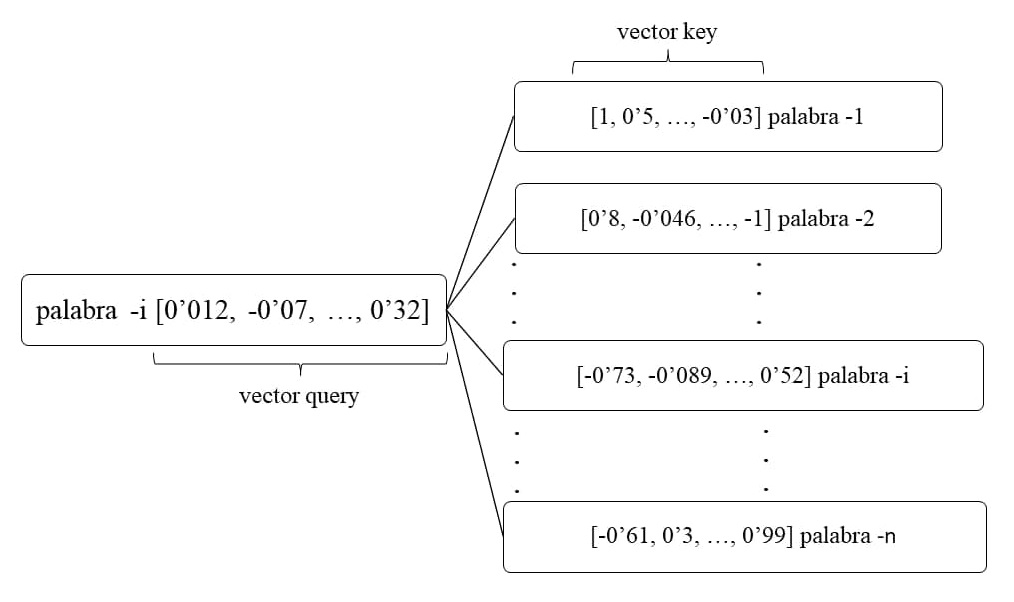
\includegraphics[width = 0.8\textwidth]{Imagenes/Bitmap/query-key.jpg}}%
	\caption{Esquema de atención query-key}%
	\label{fig:querykey}
\end{figure}

Dados dos vectores (el vector query y el vector key), matemáticamente se puede calcular su similitud hallando el coseno del ángulo que forman. Este se calcula con la siguiente fórmula:

$$
\cos(\alpha) = \frac{<q, k>}{|q|\cdot|k|}
$$
donde $<q, k>$ es el producto escalar entre ambos vectores y $|v|$ es el módulo de $v$. Asimismo es posible conocer un valor de relación entre cada palabra con todas las de la oración. La fórmula anterior puede generalizarse como sigue:

$$
similitud(q,k)=\frac{<q, k>}{e}
$$
donde $e$ es un factor de escalado prestablecido. Como lo que se busca es computar la similitud de todas los token con todos, se debe pasar la expresión anterior a forma matricial (con los vectores query de cada palabra como filas se conforma la matriz $Q$ y, análogamente, se crea la matriz $K$ con los vectores key de cada token):

$$
similitud(Q, K)=\frac{Q\cdot K^T}{e}
$$

La fórmula anterior genera otra matriz (llamada filtro de atención) cuyos elementos determinan la similitud entre las palabras, concretamente es posible afirmar que el elemento de la fila i-ésima y la columna j-ésima representa la medida de similitud entre la palabra i-ésima como query y el token j-ésimo como key. De hecho a cada fila de esta matriz se le denomina vector de atención de la palabra a la que corresponde la query, el cual indica qué palabras el modelo considera relevantes para dar contexto al token, o dicho de otra forma, a qué parte de la frase se está prestando atención.

\cite{transformers} determinan el factor de escalado como $\sqrt{d}$, donde $d$ es la dimensión del vector query (o del vector key que poseen el mismo número de componentes). Además, a cada elemento resultante del filtro de atención, le aplican la función softmax para delimitar sus valores entre 0 y 1, quedando el cálculo de similitud de la siguiente manera:

$$
similitud(Q, K)=softmax\left(\frac{Q\cdot K^T}{\sqrt{d}}\right)
$$

Como se ha comentado anteriormente, los mecanismos de atención constan de tres redes neuronales. Se han presentado la query y la key. La tercera, conocida como \textit{Value}, generará un vector (vector value) cuyos elementos representarán las características de una palabra de cara a producir el resultado esperado por el sistema. Esto se consigue permitiendo que el backpropagation le afecte en mayor medida al no introducirlo en los cálculos anteriores. Su utilidad será aplicarle la matriz de filtro, que potenciará aquellas características a las que haya que prestarle mayor atención, es decir, aquellos elementos de la matriz que tengan valores más cercanos a 1. De esta forma, el cálculo final de la matriz de atención viene dado por la siguiente expresión:

$$
atencion(Q, K, V)=softmax\left(\frac{Q\cdot K^T}{\sqrt{d}}\right)\cdot V
$$

En resumen, si contamos con tres redes neuronales que, dados los tokens, obtengan los vectores query, key y value, es posible generar la matriz de atención combinando la matriz query con la matriz key, escalando el filtro de atención resultante, aplicando la función softmax para tener valores entre 0 y 1 y, por último aplicando el filtro a la matriz value (este flujo además de quedar formalizado por la expresión anterior, viene esquematizado en la imagen \ref{fig:qkv}).

\begin{figure}[h]
	\centering%
	\centerline{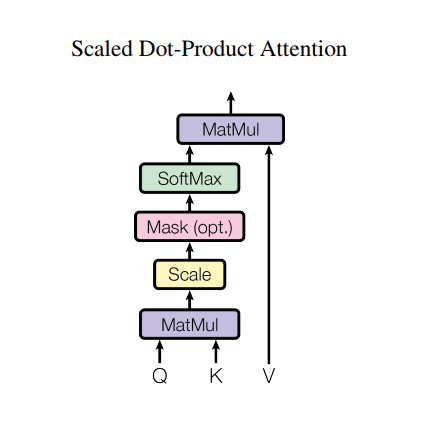
\includegraphics[width = 0.6\textwidth]{Imagenes/Bitmap/scaled-attention.png}}%
	\caption{Cálculo de atención (Query-Key-Value)}%
	Imagen extraída de \cite{transformers}
	\label{fig:qkv}
\end{figure}

No obstante, nos queda por especificar cómo se generan las matrices query, key y value. \cite{transformers} proponen la utilización de una capa lineal de neuronas, que consiste en una capa de neuronas plenamente conectadas sin función de activación. Suelen resultar extremadamente útiles cuando se desea cambiar las dimensiones de la entrada de la red neuronal.

Con este mecanismo de atención explicado, es posible conocer las características más importantes en las que el sistema debe fijarse gracias al filtro de atención. Sin embargo, existen una amplia variedad de filtros que permiten concentrarse en otro tipo de conjunto de características que podrían enriquecer la salida de nuestro componente de atención. Por ese motivo, la arquitectura transformer trabaja generando ocho matrices distintas de atención ($h = 8$), concatenándolas y reescalando la matriz final para ajustarse a las dimensiones. Este conjunto de operaciones es lo que se conoce como \textit{Multi-Head Attention} (véase la figura \ref{fig:multiattention} que resume toda la arquitectura) y se utiliza en varios puntos de la arquitectura propuesta por \cite{transformers} (véase la figura \ref{fig:transformer}).

\begin{figure}[h]
	\centering%
	\centerline{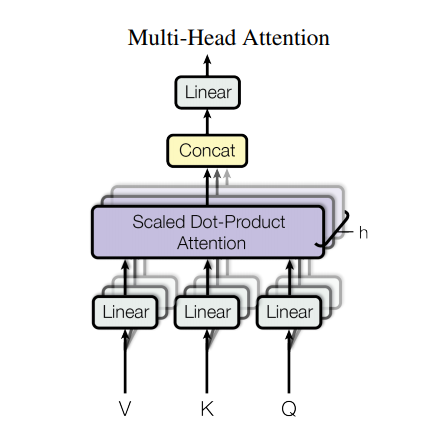
\includegraphics[width = 0.6\textwidth]{Imagenes/Bitmap/multi-head-attention.png}}%
	\caption{Multi-Head Attention}%
	Imagen extraída de \cite{transformers}
	\label{fig:multiattention}
\end{figure}

Si se analiza en detalle la figura \ref{fig:transformer}, es fácil percatarse que existen conexiones residuales, es decir, conexiones que, en lugar de ir de una componente de la arquitectura a la siguiente acaban en capas posteriores. Una de las ventajas de contar con este tipo de conexiones, es preservar parte del conocimiento de entrada, ya que conforme se profundiza y avanza en las distintas capas, la entrada se modifica considerablemente, lo que puede causar que se pierda información. Una solución a esto, es precisamente conectar los valores de entrada, no solo con la primera capa, sino también con capas ocultas de mayor profundidad, de manera que ``se refresca'' la información a la red neuronal. Para ello, basta con sumar los vectores que llegan a través de la conexión residual con los que son resultado del procesamiento de las capas anteriores. En la arquitectura que se está presentando, tras esta suma, se aplica una estandarización (cambiar la distribución de la muestra a una normal de media 0 y desviación típica 1) de los valores de la matriz resultante, a lo largo de sus columnas (las características de los tokens).

También se pueden observar componentes \textit{feed forward}, los cuales se componen de dos capas lineales de neuronas con una capa con función de activación ReLU. Así queda explicada por completo la arquitectura del codificador, y faltaría presentar una pequeña variación de la componente de Multi-Head Attention detallada anteriormente que se puede encontrar en el decodificador: el enmascaramiento. Esta técnica simplemente consiste en multiplicar al filtro de atención una matriz triagular superior con la diagonal nula para que, durante el entrenamiento, solo se tomen como entradas del decodificador las palabras que ya se han generado y no las que quedan por producir. Esta pequeña variación sirve para no introducir como entrada del codificador lo que se espera como salida.

En resumen, la arquitectura transformer se divide en codificador y decodificador. El primero recibe la entrada del sistema y el segundo recibe como input el texto que ha ido generando hasta el momento. Cuando queremos usar este tipo de redes neuronales, primero se tokeniza el texto de partida y este pasa a una capa de embeddings que extrae propiedades de las diferentes palabras. A continuación se genera el embedding posicional sumándole al vector embedding el vector de posición que incluye la información de cómo se ordenan las palabras en la frase. A continuación, estos vectores que almacenan propiedades y posición de las palabras, entran por el módulo de Multi-Head Attention, del que se obtiene la matriz de atención. A esta se le suman los embedding posicionales y luego se estandariza la matriz. Luego, el resultado pasa por la componente feed forward y, de nuevo, volvemos a utilizar una conexión residual para sumarle al resultado de dicha capa la matriz de atención estandarizada. Al estandarizar el resultado se produce la salida del codificador, la cual se incluye como query y key de un módulo de Multi-Head Attention del decodificador. La clave de esta componente será el resultado de obtener la matriz de atención de la entrada del decodificador. El último paso de antes de la salida es de nuevo una capa feed forward, seguida de una conexión residual. Por último, la salida del decodificador llega a una capa lineal de neuronas que tendrá tantas neuronas como el tamaño del vocabulario de salida. Con esta capa, se calculan los pesos asignados a cada palabra del vocabulario que, al pasarlos por la función softmax final, se convierten en probabilidades que pueden ser interpretadas fácilmente y nos indican el token que el sistema recomienda generar.